\documentclass[twocolumn]{article}

\usepackage[margin=1in]{geometry}

\usepackage{pbalance}
\usepackage{listings}
\usepackage{appendix}
\usepackage{hyperref}
\usepackage{booktabs}
\usepackage{adjustbox}
\usepackage{placeins}


% Default fixed font does not support bold face
\DeclareFixedFont{\ttb}{T1}{txtt}{bx}{n}{12} % for bold
\DeclareFixedFont{\ttm}{T1}{txtt}{m}{n}{12}  % for normal

% Custom colors
\usepackage{color}
\definecolor{deepblue}{rgb}{0,0,0.5}
\definecolor{deepred}{rgb}{0.6,0,0}
\definecolor{deepgreen}{rgb}{0,0.5,0}

% Python style for highlighting
\newcommand\pythonstyle{\lstset{
language=Python,
basicstyle=\ttm,
morekeywords={self},              % Add keywords here
keywordstyle=\ttb\color{deepblue},
emph={MyClass,__init__},          % Custom highlighting
emphstyle=\ttb\color{deepred},    % Custom highlighting style
stringstyle=\color{deepgreen},
commentstyle=\ttfamily, % Change comment font to typescript
frame=tb,                         % Any extra options here
showstringspaces=false
}}
% Python environment
\lstnewenvironment{python}[1][]
{
\pythonstyle
\lstset{#1}
}
{}




\begin{document}

\title{Regression and Clustering Analysis of US Political Instability}
\author{Jichao Yang}
\maketitle

\begin{abstract}
    This report examines the use of regression and clustering algorithms to predict political instability in the US using historical data. Three models—linear regression, random forest, and a neural network—are trained and compared. Principal Component Analysis and clustering techniques explore latent patterns. Results show that political instability follows nonlinear trends, with the neural network performing best but struggling with extreme events. Clustering suggests models capture meaningful structures beyond memorization. The findings highlight the importance of preliminary data analysis and model selection in larger scale machine learning problems.
\end{abstract}

\section*{Introduction}
This report aims to find correlations between socio-political data and political instability in the United States. The report will approach the problem by comparing the performance of various supervised and unsupervised machine learning algorithms. The analysis will also examine how effective the algorithms extract patterns and knowledge from the dataset, as against simply memorizing historical facts. Finally, this report will discuss how the methodology of our analysis can be extended to larger scales and real world problems.

\section{Data Wrangling}
\subsection{Data Sources}
The United States Political Violence (USPV) dataset is used to calculate the yearly political instability index in US. Independent variables include population, economic, political, and health data, sourced from the United States Census Bureau and pre-processed datasets. A list of all variables and their interpolated values between 1901 and 1910 can be found in Appendix A.

\subsection{Interpolation}
The datasets require cleaning and interpolation before analysis. Specifically, there are numerous cases where multiple entries of data are all collected within the same year, while there are also time periods when no data is recorded. A single value for each variable is generated for all years, by first averaging all entries from the same year, and then linearly interpolating data for the years with no entry.

The political instabilitiy index is calculated annually as the log-transformed sum of people killed in instability events per one million population per 5 years. Years with no recorded deaths are concentrated overwhelmingly prior to 1850, and agree with a general low trend of annual death counts (see Figure \ref{fatalities}). Empty entries are hence interpreted as years with 0 death count. In addition, two entries in the dataset are of the type 'Compilation,' and have significantly higher value than the rest of the dataset. The two datapoints are removed as outliers. Finally, all variables except year and the instability index are normalized.


\section{Exploratory Data Analysis}
\subsection{Feature Engineering}
Given that the dataset is a time series, there are certain features that might work well to predict the outcome other than the variables themselves. For example, if life expectancy is an important predictor in political instability, would a sudden increase in life expectancy affect political instability as well? To answer the question, 8 engineered features are added to the dataset, each equalling the amount of yearly change of a variable.

\subsection{Nonlinearity}
A crude analysis of the relationship between the independent and the dependent variables can benefit complex model training significantly. By plotting the instability index against different variables, we see that some relationships have a linear trend, others have a non-linear trend, and certain variables have no immediately obvious relationship with the dependent variable. See Figure \ref{linear} and \ref{nonlinear} for examples of such varaibles.

A seeming lack of relationship for certain variables might indicate that the variable works with other variables to generate the outcome. This motivates training the dataset on a random forest model. A fully connected neural network is also useful for capturing nonlinear trends. Finally, a simple linear regression will act as the control group to compare against the nonlinear algorithms.

\section{Regression}
Preliminary analysis in Subsection 2.2 motivates us to choose models that work well with nonlinear data. In this section, we will closely analyze the performance of each regressor, and interpret the corresponding results.
\subsection{Implementation}
The normalized dataset is trained on three models: a simple linear regression, a random forest, and a fully connected feed-forward neural network. The best hyperparameters for random forest pruning and the best architecture for the neural network are found using GridSearchCV. In order to determine the effectiveness of the engineered features, all three models are trained on both the original dataset and the feature engineered dataset.

Considering that the three models are based on different principles and have vastly different architectures, the best metric for cross-comparsion of the training accuracy is the Mean-Squared Error (MSE) between the predicted instability and the observed instability. In addition, a $R^2$ score is calculated to measure how well the model correlates between instability and the independent variables. All models are trained and tested on different folds of the dataset, and the metrics are calculated based on the models' performance on the testing dataset.

\subsection{Results}
Table \ref{engineered_results} shows the model's performance on the unengineered dataset with only the original 8 variables. The neural network's optimal architecture is $[8,16,64,1]$.
\FloatBarrier
\begin{table}[h!]
    \centering
    \begin{tabular}{lcc}
        \toprule
        Model & MSE & $R^2$ \\
        \midrule
        Linear Regression & 0.495 & 0.771 \\
        Random Forest & 0.287 & 0.838 \\
        Neural Network & 0.157 & 0.912 \\
        \bottomrule
    \end{tabular}
    \caption{Performance on Unengineered Dataset}
    \label{engineered_results}
\end{table}
\FloatBarrier
Table \ref{results} shows the model's performance on the unengineered dataset with only the original 8 variables. The neural network's optimal architecture is $[16,32,32,32,1]$.

\begin{table}[h!]
    \centering
    \begin{tabular}{lcc}
        \toprule
        Model & MSE & $R^2$ \\
        \midrule
        Linear Regression & 0.367 & 0.830 \\
        Random Forest & 0.354 & 0.801 \\
        Neural Network & 0.166 & 0.906 \\
        \bottomrule
    \end{tabular}
    \caption{Performance on Engineered Dataset}
    \label{results}
\end{table}

\subsection{Performance Analysis}
Based on the performance metrics, it is evident that the dataset is nonlinear. Linear regression fails to capture any nonlinear relationships between the variables, and hence have low $R^2$ value for both the engineered and unengineered dataset. Random forest performs better than linear regression, but the neural network model performs best on both the engineered and unengineered dataset, having $R^2$ values larger than 0.9 in both cases.

Interestingly, linear regression is the only model that performs better on the engineered dataset than the unengineered one. We suspect that two factors cause this difference. First, some nonlinearity of the dataset can be partially inferred through the engineeered variables, hence the linear model can refect the nonlinear relationships with the engineered dataset. Second, the engineered dataset have twice as much variables as the unegineered dataset. The bloated dataset very likely has introduced more noise than signal. Considering that random forest and neural network both have much more coefficients on a wider dataset, training is much less efficient and both models are more prone to overfitting.

\subsection{Pattern Extraction}
High accuracy does not necessarily mean good pattern. For larger models such as the neural network, is the model simply memorizing the data entries? Or is it memorizing US history? Or is it really finding some interesting sociological pattern in the data?

Figure \ref{nn_prediction} and \ref{nn_error} shows the neural network's prediction and error against the observed data, when trained on the unengineered set. The prediction percent error graph shows a general stable trend, with sudden spikes of large error around specific time periods. This might indicate that the neural network finds a common pattern across different years, but fails to predict political instability during extreme times. Indeed, the four largest spikes all correspond to the time period when the United States is in some form of crisis. The first two spikes correspond to the Panic of 1837 and the Great Depression, the largest two economic recessions in American history. The third and fourth spike correspond to World War I and II. The model's inability to predict extreme and unusual scenarios indicates that the regression likely has picked up meaningful patterns from the training dataset, as against to overfitting and 'memorizing' the dataset.

\section{Dimension Reduction}

\subsection{Principle Component Analysis}
If the engineered dataset has too much noise for the models to train efficiently, can we improve the prediction accuracy on a dataset with reduced dimensions?

Before choosing a dimension reduction algorithm, it is worth noting that the dataset is exceptionally small. The entire dataset is composed of about only 100 entries, which is much less than the minimum requirement for most dimension reduction algorithms. For this reason, we pick Principal Component Analysis (PCA) as the method to reduce the dataset to 2 dimensions. Figure \ref{pca} shows the dataset in reduced dimension, the coloring of which shows political instability index.

\subsection{Results}
After applying PCA to reduce the dataset to 2 dimensions, we trained a neural network on the two principal components to predict the instability index. GridSearchCV is used to determine the best architecture for the neural network, in this case $[2,8,16,8,1]$. Table \ref{pca_pred} is the model's performance metrics compared to the neural network trained on the entire dataset.

\begin{table}[h!]
    \centering
    \begin{tabular}{lcc}
        \toprule
        Dataset & MSE & $R^2$ \\
        \midrule
        PCA Dataset & 0.238 & 0.866 \\
        Original Dataset& 0.166 & 0.906 \\
        \bottomrule
    \end{tabular}
    \caption{Neural Network Performance}
    \label{pca_pred}
\end{table}

The neural network performs worse on the transformed dataset than the original dataset. This is likely due to the inevitable signal loss during dimension reduction. The neural network loses a portion of the useful information from the independent variables that can contribute to predicting the dependent variable.

\section{Unsupervised Classification}
\label{unsup_class}
Aside from using dimension reduction to predict instability index, we can also apply unsupervised learning algorithms on the dimension reduced dataset, and see if any learnt clusters correspond with the instability index.
\subsection{Implementation}
The classification models we selected are K-Means Clustering and DBSCAN Clustering. There are two reasons that motivate this choice. First, the dataset is relatively small. This rules out clustering algorithms whose performance require a minimum number of data entries. Furthermore, referring to the PCA analysis (Figure \ref{pca}), meaningful clusters in the dataset does not always necessarily have spherical shapes. DBSCAN is especially useful for spotting non-spherical clusters.
\subsection{Results}
The visualized clusters of both PCA and DBSCAN can be found in Figure \ref{kmeans} and \ref{dbscan}. K-Means Clustering and DBSCAN Clustering report a silhouette score of 0.621 and 0.501, respectively.
\subsection{Analysis}
Both the silhouette score and the visualizations of the clusterings indicate that K-Means clusters the PCA dataset better than DBSCAN. Optimizing the DBSCAN hyperparameters is largely futile towards increasing the silhouette score, with larger $\epsilon$ values generating too few clusters ($\leq  2$), and smaller $\epsilon$ causing a significant ($\geq 25 \%$) portion of the dataset to be marked as outliers.

In contrast, plotting the inertia against the number of clusters in K-Means shows a clear elbow point, and yields better results consistenly as compared to DBSCAN. Furthermore, the optimal DBSCAN model arrived at the same number of clusters as the elbow point in K-Means Clustering. This shows that the manual choice of $k$ in K-Means Clustering is reasonable in this case.

\section{Cluster Analysis}
Results from Section \ref{unsup_class} are learnt without supervision, meaning that the model does not have access to the instability index when training. We plot the Kernel Density Estimation (KDE) of each variable grouped by clusters, to see if the learnt clusters correlate to any properties in the data.
\subsection{Instability Clusters}
The KDE of instability index grouped by clusters is shown in Figure \ref{kde_instab}. The plot yields ambivalent results. On the one hand, data from the same cluster do share a similar instability index. This can also be cross-referenced from comparing Figure \ref{pca}, \ref{kmeans}, and \ref{dbscan}. Yet on the other hand, a given instability score does not determine the cluster of its data entry. In other words, multiple clusters share the same instability score ranges. This suggests that the clusters are a necessary but insufficient variable when predicting the instability index.
\subsection{Year Clusters}
The KDE of the year in which the data is recorded, grouped by clusters is shown in Figure \ref{kde_year}. Not only does each cluster share similar years, each year value also coarsely correlate to one unique cluster. This is significant in that year is not accessible to the model either during K-Means Clustering or PCA. K-Means Clustering is able to determine a correlation between the features of the data and the year of the data entry is learnt by K-Means Clustering, without supervision from the data year value itself. The clusters found using K-Means is both necessary and sufficient when predicting the instability index, showing that the unsupervised learning has indeed picked up new patterns and features from the dataset.

\section{Conclusion}
This report compares and summarizes the result of (1) applying linear regression, random forest, and neural network as regressors on the US political stability dataset, (2) applying PCA for dimension reduction on the independent variables, (3) applying K-Means and DBSCAN clustering on the PCA component dataset, and (4) correlating unsupervised clusters to features of the dataset. Fully connected simple neural network proves to be the best regressor due to its capability to handle dataset non-linearity, and K-Means Clustering infers meaningful patterns from the dataset without supervision.

In real life situations, the complexity of the problem and of the dataset often allows a much wider selection of available models and approaches. Besides accuracy and correlation, the choices of metrics that compare different models are usually limited: for example, comparing cross-entropy loss of one model against mean squared error loss of another model is rarely statistically interesting.

This report circumvents the issue by carefully selecting the most interesting models based on preliminary data analysis that does not involve machine learning algorithms. Key aspects of the dataset, including its concavity and nonlinearity, significantly motivated the optimal model choices. Such is also the case for larger-scale, real-life scenarios. Lacking a good method to easily pick a fitting model, it comes to experience, industry standard, and careful observation of the dataset to find the best solution.


\newpage
\onecolumn
\section*{Appendices}
\begin{appendices}

\section{Sample Dataset}
    \begin{adjustbox}{angle=90, center}
    \begin{tabular}{llllllllll}
        \toprule
         & instability & immigration & height & evi & polarization & population & wagegdpratio & hsus & age \\
        \midrule
        1901 & 1.62 & 13.8 & 170.33 & 1474.49 & 0.85 & 77813801.0 & 0.65 & 30.71 & 50.42 \\
        1902 & 1.44 & 13.9 & 170.5 & 1566.71 & 0.86 & 79415434.0 & 0.65 & 31.29 & 50.57 \\
        1903 & 0.54 & 13.99 & 170.67 & 1667.19 & 0.87 & 81017066.0 & 0.64 & 31.88 & 50.74 \\
        1904 & 0.55 & 14.09 & 170.89 & 1739.17 & 0.88 & 82618699.0 & 0.63 & 32.22 & 50.9 \\
        1905 & 0.12 & 14.2 & 171.1 & 1850.34 & 0.89 & 84220332.0 & 0.61 & 32.53 & 51.06 \\
        1906 & 0.51 & 14.34 & 171.33 & 1965.17 & 0.9 & 85821965.0 & 0.6 & 33.11 & 51.2 \\
        1907 & 0.53 & 14.48 & 171.56 & 2051.36 & 0.89 & 87423598.0 & 0.61 & 33.72 & 51.35 \\
        1908 & 0.59 & 14.58 & 171.78 & 2182.49 & 0.88 & 89025230.0 & 0.61 & 34.03 & 51.54 \\
        1909 & 0.53 & 14.67 & 172.02 & 2325.6 & 0.87 & 90626863.0 & 0.61 & 34.35 & 51.72 \\
        1910 & 0.99 & 14.62 & 172.19 & 2419.6 & 0.86 & 92228496.0 & 0.6 & 34.94 & 51.89 \\
        \bottomrule 
    \end{tabular}\\
\end{adjustbox}
\begin{center}
Table 3: Interpolated data from 1901 to 1910
\end{center}
\newpage



\section{Graphs}
\FloatBarrier
\begin{figure}[h!]
    \centering
    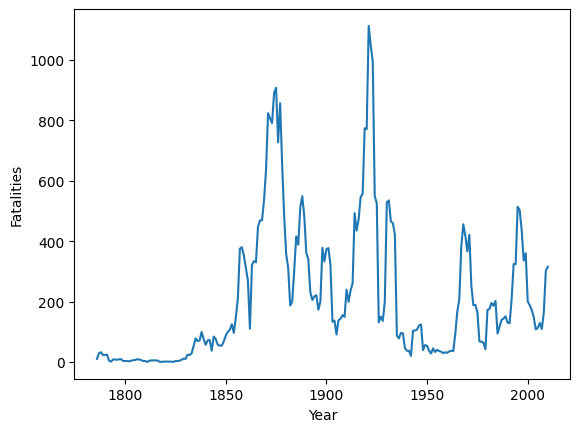
\includegraphics[width=0.75\textwidth]{images/fatalities.png}
    \caption{Interpolated Annual Political Violence Death Count}
    \label{fatalities}
\end{figure}
\FloatBarrier
\begin{figure}[h!]
    \centering
    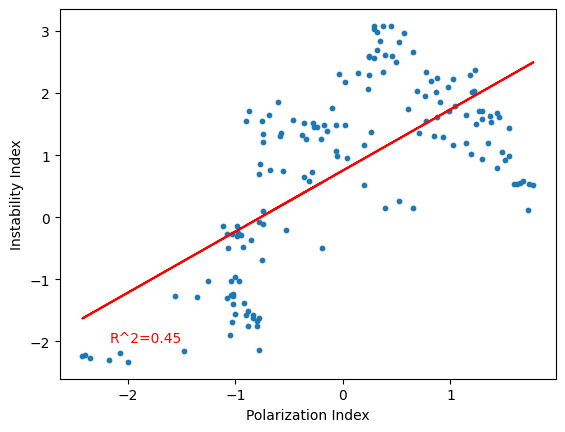
\includegraphics[width=0.75\textwidth]{images/linear.png}
    \caption{Linear Relationship between Instability and Polarization}
    \label{linear}
\end{figure}
\FloatBarrier
\begin{figure}[h!]
    \centering
    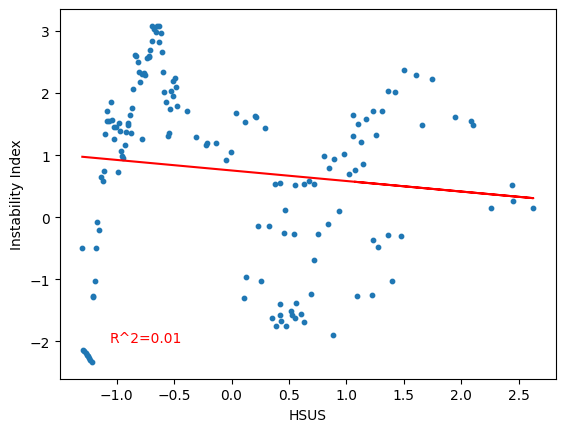
\includegraphics[width=0.75\textwidth]{images/nonlinear.png}
    \caption{Nonlinear Relationship between Instability and HSUS}
    \label{nonlinear}
\end{figure}
\FloatBarrier
\begin{figure}[h!]
    \centering
    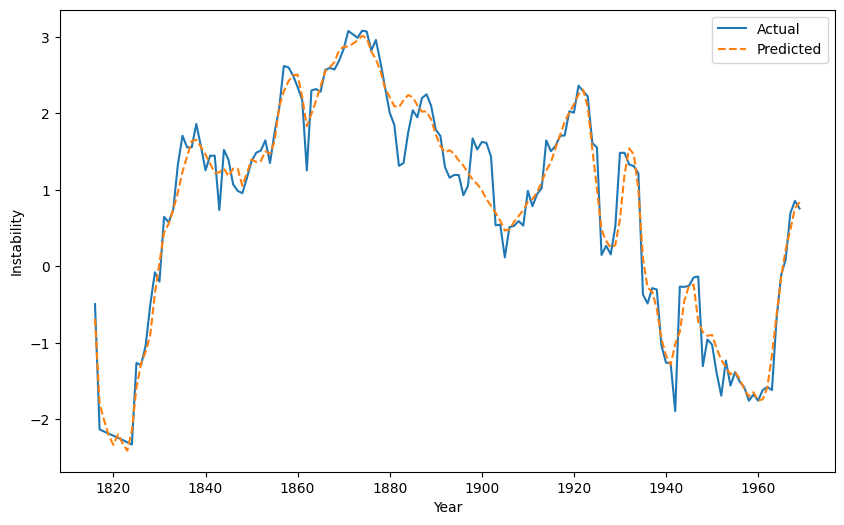
\includegraphics[width=0.75\textwidth]{images/predicted_instability.png}
    \caption{Actual vs Predicted Instability, Neural Network}
    \label{nn_prediction}
\end{figure}
\FloatBarrier
\begin{figure}[h!]
    \centering
    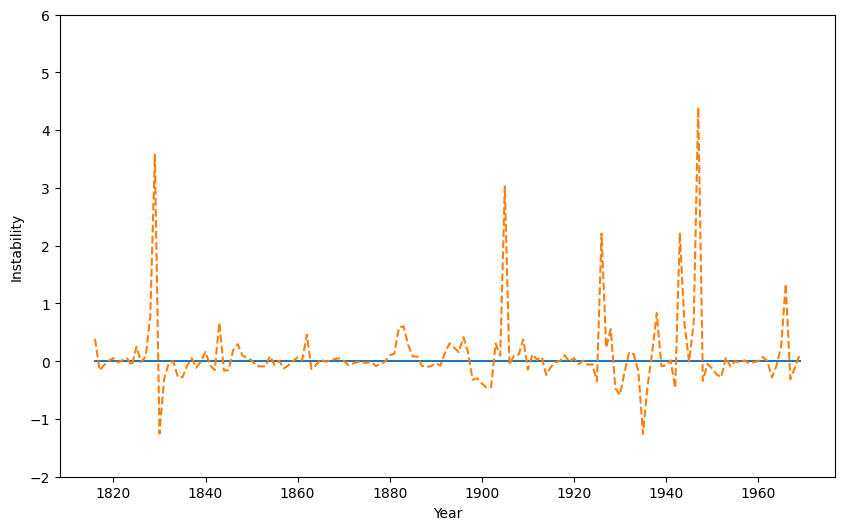
\includegraphics[width=0.75\textwidth]{images/predicted_error.png}
    \caption{Instability Prediction Perent Error, Neural Network}
    \label{nn_error}
\end{figure}
\FloatBarrier
\begin{figure}[h!]
    \centering
    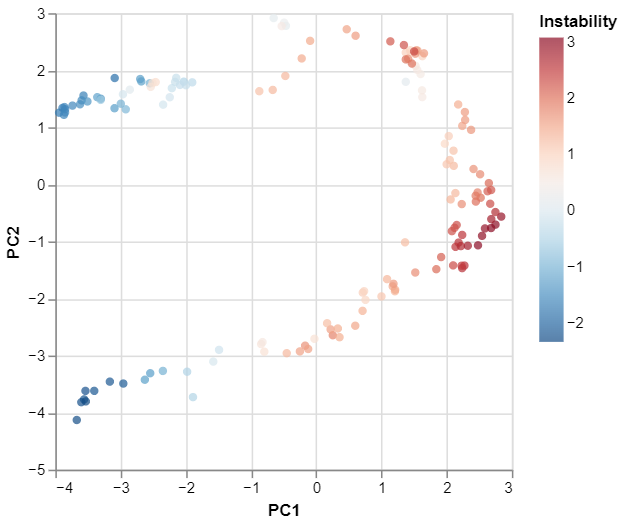
\includegraphics[width=0.75\textwidth]{images/pca.png}
    \caption{PCA Reduced Dimension Dataset}
    \label{pca}
\end{figure}
\FloatBarrier
\begin{figure}[h!]
    \centering
    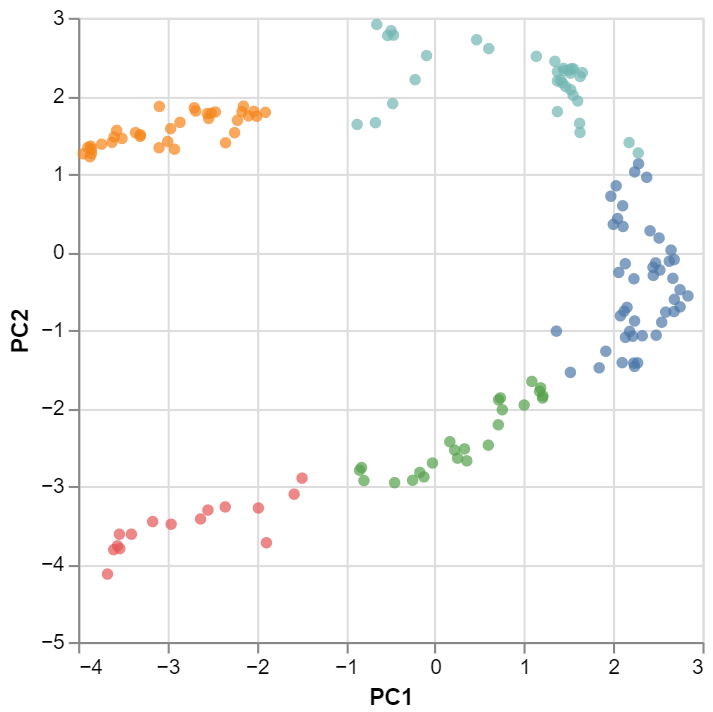
\includegraphics[width=0.75\textwidth]{images/kmeans.png}
    \caption{K-Means Clustering of PCA Dataset}
    \label{kmeans}
\end{figure}
\FloatBarrier
\begin{figure}[h!]
    \centering
    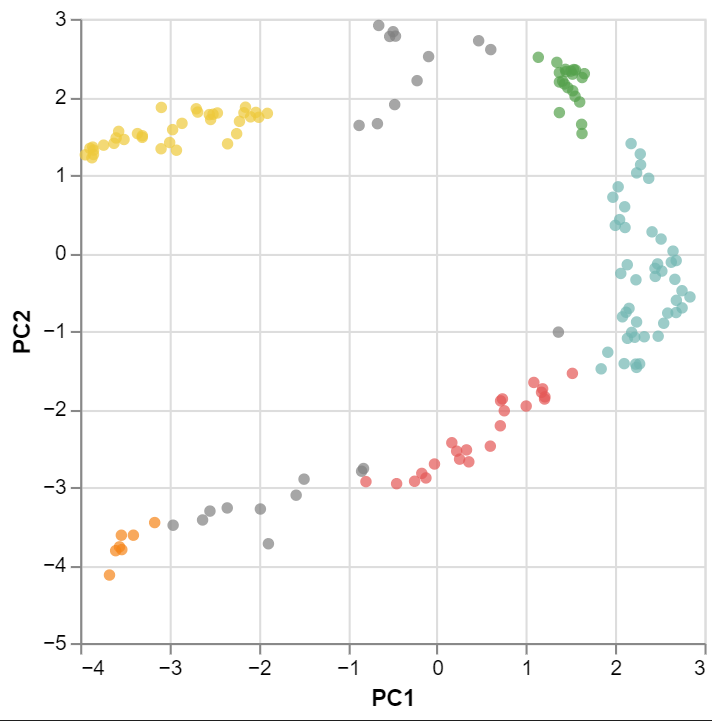
\includegraphics[width=0.75\textwidth]{images/dbscan.png}
    \caption{DBSCAN Clustering of PCA Dataset}
    \label{dbscan}
\end{figure}
\FloatBarrier
\begin{figure}[h!]
    \centering
    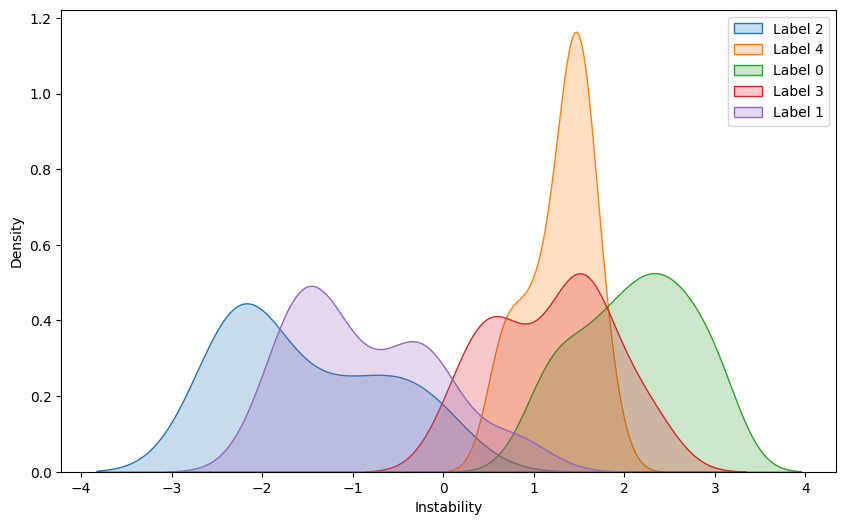
\includegraphics[width=0.75\textwidth]{images/kde_instab.png}
    \caption{Kernel Density Estimation of Instability Index by Clusters}
    \label{kde_instab}
\end{figure}
\FloatBarrier
\begin{figure}[h!]
    \centering
    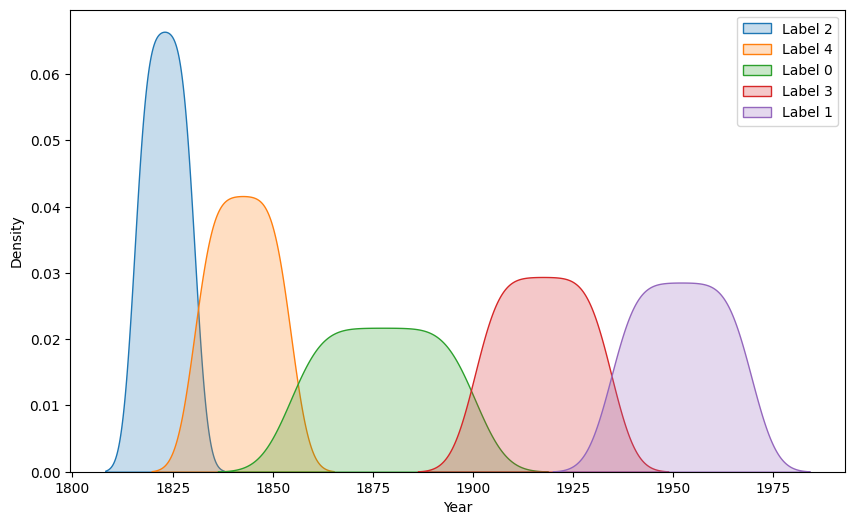
\includegraphics[width=0.75\textwidth]{images/kde_year.png}
    \caption{Kernel Density Estimation of Year by Clusters}
    \label{kde_year}
\end{figure}
\FloatBarrier
\newpage

\section{Code}
The code below can be of reference in order to replicate the results of this report.
\subsection{Data Wrangling}
\begin{python}
def wrangle(file, name):
    '''Function to wrangle data'''
    # Take mean for years with multiple values
    df = df.groupby('year', as_index=False).mean()
    # What are the missing years?
    all_years = np.arange(df['year'].min(),\
    df['year'].max() + 1)
    missing_years = [int(y) for y in all_years \
    if y not in df['year'].values]
    # Interpolate missing years
    all_years = pd.DataFrame({'year': all_years})
    df = pd.merge(all_years, df, on='year', how='left')
    df['value'] = df['value'].interpolate(method='linear')
    return missing_years

# read and interpolate years linearly
all_years = np.arange(df_pop['year'].min(),\
df_pop['year'].max() + 1)
all_years = pd.DataFrame({'year': all_years})
df_pop = pd.merge(all_years, df_pop, on='year', how='left')
df_pop = df_pop.interpolate(method='linear')
df_pop['population'] = np.round(df_pop['population'], 0)

# calculate fatalities
df['year'] = df['year'].astype(int)
# Take mean for years with multiple values
df = df.groupby('year', as_index=False).sum()
# What are the missing years?
all_years = np.arange(df['year'].min(), df['year'].max() + 1)
missing_years['instability'] = \
[int(y) for y in all_years if y not in df['year'].values]

# Calculate Instability index
# Calculate the 5-year aggregative fatalities
df = df.fillna(0)
df['fatalities'] = df['fatalities'].rolling(5).sum()
df['population'] = df['population'].rolling(5).sum()
# Log cannot take 0 so we need to add 0 entries with 1
df.loc[df['fatalities']==0, 'fatalities'] = 1
df['instability'] = np.log(
    df['fatalities'] *1e6 * 5 / df['population'])
df = df.drop(columns=['fatalities', 'population'])
\end{python}
\newpage
\subsection{Exploratory Data Analysis}
\begin{python}
def plot(col):
    '''
    plot index against selected variable
    '''
    X = df[[col]]
    y = df['instability']
    model = LinearRegression()
    model.fit(X, y)
    y_pred = model.predict(X)
    r2 = model.score(X, y)
    plt.scatter(X, y)
    plt.plot(X, y_pred, color='red')
    plt.text(0.1, 0.1, f'R^2={r2:.2f}')
\end{python}

\subsection{Regression}
The implementation for different models are largely the same, with only minor differences in model selection and hyperparameter choices. Hence only the code for the neural network model will be displayed.
\begin{python}
c = [c for c in df.columns if c != \
'instability' and c[-5:] != '_diff'] 
X = df[c]
# Split the data into training and testing sets
X_train, X_test, y_train, y_test = \
train_test_split(X, y, test_size=0.2)
# Create and fit the neural network model on the training set
nn_model = MLPRegressor(hidden_layer_sizes=(32,32,32),\
max_iter=1000)
nn_model.fit(X_train, y_train)
y_train_pred = nn_model.predict(X_train)
y_test_pred = nn_model.predict(X_test)
# Calculate metrics
test_r_squared = nn_model.score(X_test, y_test)
test_mse = mean_squared_error(y_test, y_test_pred)
\end{python}
\subsection{Dimension Reduction}
\begin{python}
# Apply PCA
pca = PCA(n_components=2)
df_pca = pca.fit_transform(df)
df_pca = pd.DataFrame(df_pca, \
columns=['PC1', 'PC2'], index=df.index)
df_pca['instability'] = df_diff['instability']
\end{python}
\newpage
\subsection{Unsupervised Classification}
\begin{python}
# Use the elbow method to find the optimal number of clusters
inertia = []
for n in range(1, 11):
    kmeans = KMeans(n_clusters=n)
    kmeans.fit(X)
    inertia.append(kmeans.inertia_)
# Use KneeLocator to find the elbow point
kneedle = KneeLocator(range(1, 11), inertia,\
curve='convex', direction='decreasing')
optimal_clusters = kneedle.elbow
kmeans = KMeans(n_clusters=5)
df['kmeans_labels'] = kmeans.fit_predict(X)

# Apply DBSCAN clustering
dbscan = DBSCAN(eps=0.4, min_samples=5)
df['dbscan_labels'] = dbscan.fit_predict(X)
\end{python}

\end{appendices}


\end{document}